\documentclass[12pt]{article}

% Set the page to be letter paper and have small margins
\usepackage{geometry}
\geometry{letterpaper, left=15mm, right=15mm, top=15mm, bottom=20mm}

% LuaLaTeX font setup
\usepackage{fontspec}
\usepackage{unicode-math}

% Text font
\setmainfont{DejaVu Serif}

% Math font
\setmathfont{STIX Two Math}

\allowdisplaybreaks[1]

\usepackage{standalone}
\usepackage{parskip}
\usepackage{amsmath}
\usepackage{amsthm}
\usepackage{multicol}
\usepackage{graphicx}
\usepackage{pgfplots}
\pgfplotsset{compat=1.18}
\usepackage{cancel}
\usepackage{xcolor}
\usepackage[utf8]{inputenc}
\usepackage{float}
\usepackage{graphicx}
\usepackage{pdfpages}
\usepackage{booktabs}

% \usepackage{hyperref}
\usepackage{cleveref}


\usepackage{titlesec}
\titleformat{\section}{\normalfont\normalsize\bfseries}{\thesection.}{1em}{}
\titleformat{\subsection}{\normalfont\normalsize\bfseries\itshape}{\thesubsection}{1em}{}

\usepackage{enumitem}
\setlist[enumerate, 1]{label=\textbf{\arabic*}.}
\setlist[enumerate, 2]{label=\textbf{\alph*}.}

% \usepackage[style=ieee]{biblatex}
% \addbibresource{src/refs.bib}

\makeatletter
\newcommand{\course}[1]{\def\@course{#1}}

\renewcommand{\maketitle}{
    \noindent
    \@author \hfill \@course \newline
    \@date
    \begin{center}
        \large\textbf{\@title}
    \end{center}
    \bigskip
}

\author{Jeffrey Morris}
\course{MATH 4306-010}
\date{\today}


\begin{document}
\begin{gather*}
    f(-x)=-f(x) \Rightarrow f(x) \text{ is odd.} \\
    \text{Since $f(x)$ is odd: $a_0 = \boxed{0}$ and $a_n=\boxed{0}$}
\end{gather*}
\begin{align*}
    b_n & =\frac{1}{L}\int_{-L}^{L}f(x)\sin\left(\frac{n\pi x}{L}\right)\,dx   \\
    b_n & =\frac{1}{2}\int_{-2}^{2}f(x)\sin\left( \frac{n\pi x}{2} \right)\,dx \\
    b_n & =1\int_{0}^{2}1\cdot\sin\left( \frac{n\pi x}{2} \right)\,dx          \\
    b_n & =\frac{2}{n\pi}\left.\cos\left( \frac{n\pi x}{2} \right)\right|_0^2  \\
    b_n & =\frac{-2}{n\pi}\left( \cos(n\pi) -\cos(0) \right)                   \\
    b_n & =\frac{-2}{n\pi}\left( (-1)^n -1 \right)                             \\
    b_n & =
    \boxed{
        \begin{cases}
            0,              & \text{if $n$ is even} \\
            \frac{4}{n\pi}, & \text{if $n$ is odd}
        \end{cases}
    }
\end{align*}
\begin{align*}
    f(x) & =a_0+\sum_{n=1}^{\infty}\left( a_n \cos\left( \frac{n\pi x}{L} \right) + b_n\sin\left( \frac{n\pi x}{L} \right) \right) \\
    f(x) & =\boxed{\sum_{n=\text{odd}}^{\infty}\left( \frac{4}{n\pi}\sin \left( \frac{n\pi x}{2} \right)\right)}
\end{align*}
\begin{center}
    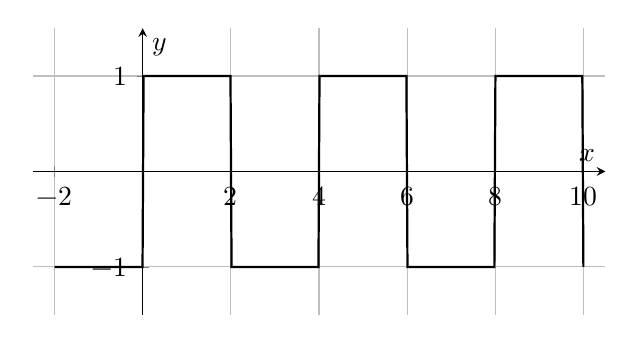
\begin{tikzpicture}
        \begin{axis}[
                axis lines=middle,
                grid=both,
                scale only axis=true,
                width=.6\textwidth,
                height=0.3\textwidth,
                xmin=-2.5, xmax=10.5,
                ymin=-1.5, ymax=1.5,
                xlabel={$x$}, ylabel={$y$},
                samples=500,
                domain=-2:10,
            ]
            \addplot[thick]{
                (mod(x+2,4)-2 < 0)*(-1)
                + (mod(x+2,4)-2 > 0)*( 1)
            };
        \end{axis}
    \end{tikzpicture}
\end{center}
\end{document}